\documentclass[prl,showpacs,twocolumn,superscriptaddress,floatfix,10pt,footinbib]{revtex4-2}

\usepackage{setspace} 
\usepackage[utf8]{inputenc}
\usepackage{float}
\usepackage{amsmath, amssymb, amsfonts, bm, bbm}
\usepackage{graphicx}
\usepackage{multirow}
\usepackage{booktabs}
\usepackage[usenames,dvipsnames]{color}
\allowdisplaybreaks
\usepackage{xcolor}
\definecolor{Tiffany}{rgb}{0, 0.7, 0.7}
\definecolor{DarkGreen}{rgb}{0, 0.4, 0}
\usepackage[colorlinks=true,
breaklinks=true,
urlcolor=magenta,
linkcolor=magenta,
citecolor=Tiffany]{hyperref}

\usepackage{orcidlink}

\newcommand{\be}{\begin{equation}}
\newcommand{\ee}{\end{equation}}
\newcommand{\ba}{\begin{align}}
\newcommand{\ea}{\end{align}}
\newcommand{\nt}{\notag\\}

\newcommand{\gr}[1]{{\color{DarkGreen}#1}}
\newcommand{\fk}[1]{{\color{blue}[FK: #1]}}
\newcommand{\tr}[1]{{\color{magenta}[TR: #1]}}

\begin{document}

\title{$H$ dibaryon and its cousins from SU(6)-constrained baryon-baryon interaction}

\begin{abstract}

We constrain the $S$-wave baryon-baryon interaction using SU(6) symmetry within a nonrelativistic effective field theory. The most general leading-order Lagrangian contains two independent parameters, which we determine using physical $NN$ and lattice QCD $\Omega\Omega$ scattering lengths. This framework allows for parameter-free predictions in the strangeness $S=-2$ sector relevant to the $H$ dibaryon. Solving the coupled-channel scattering problem, we identify two bound states below the $\Lambda\Lambda$ threshold, one deeply bound and one shallow, along with resonances near the $\Sigma\Sigma$ and $\Sigma^*\Sigma^*$ thresholds. We demonstrate that these poles result in distinct enhancements in $\Lambda\Lambda$ invariant mass distributions, suggesting that the $H$ dibaryon exists as a multichannel bound state and providing clear signatures for experimental verification.

\end{abstract}

\newcommand{\ucas}{\affiliation{School of Physical Sciences, University of Chinese Academy of Sciences, Beijing 100049, China}}
\newcommand{\itp}{\affiliation{Institute of Theoretical Physics, Chinese Academy of Sciences, Beijing 100190, China}}
\newcommand{\scnt}{\affiliation{Southern Center for Nuclear-Science Theory (SCNT), Institute of Modern Physics,\\ Chinese Academy of Sciences, Huizhou 516000, China}}

\author{Tao-Ran Hu\orcidlink{0009-0003-9720-0171}}\email{hutaoran21@mails.ucas.ac.cn}\ucas\itp
\author{Feng-Kun Guo\orcidlink{0000-0002-2919-2064}}\email{fkguo@itp.ac.cn}\itp\ucas\scnt

\maketitle

Understanding the dynamics of baryon-baryon interactions remains a central problem in low-energy quantum chromodynamics (QCD), with particular relevance to the possible existence of exotic multibaryon states~\cite{Dyson:1964xwa, Locher:1985nu, Epelbaum:2008ga, Clement:2016vnl, Gal:2016boi}. Among these, the strangeness $S=-2$ sector has attracted sustained attention following the long-standing prediction of the $H$ dibaryon~\cite{Jaffe:1976yi}. Its nature---whether deeply bound~\cite{Jaffe:1976yi, Balachandran:1985fb, Yost:1985mj}, weakly bound near threshold~\cite{Straub:1988mz, Kodama:1994np, Nakamoto:1997gh, Shen:2000qs, NPLQCD:2010ocs, Inoue:2010es, Beane:2011zpa, NPLQCD:2011naw, Haidenbauer:2011ah, Haidenbauer:2011za, Inoue:2011ai, Francis:2018qch, Green:2021qol}, or virtual or resonant (quasi-bound)~\cite{Oka:1983ku, Beane:2011zpa, Shanahan:2011su, Haidenbauer:2011ah, Haidenbauer:2011za, Inoue:2011ai, Haidenbauer:2015zqb, Yamaguchi:2016kxa, HALQCD:2019wsz}---is still under active debate. Despite extensive theoretical and experimental efforts, the existence and properties of the $H$ dibaryon remain unsettled, and no conclusive evidence for the $H$ dibaryon has been observed so far, even after dedicated searches in hypernuclear decays, hadron-induced reactions, and high-energy processes~\cite{Iijima:1992pp, BNLE836:1997dwi, E885:2000ped, Takahashi:2001nm, Yoon:2007aq, Belle:2013sba}\footnote{A possibility of finding the $H$ dibaryon in radiative capture reaction $\Lambda\Lambda\to\gamma H$ was proposed in Ref.~\cite{Hikota:2015dba}.}. Yet, the observation of the $_{\Lambda\Lambda}^{~~6}$He hypernucleus has been reported~\cite{Takahashi:2001nm}, which is often interpreted as constraining the lower limit of the $H$ dibaryon mass to around 2223.7~MeV at a 90\% confidence level; however, recent work~\cite{Gal:2024nbr} argues that this constraint alone may still not exclude a deeply bound $H$ dibaryon. The structure of light $S=-2$ hypernuclei and its implications for hyperon-hyperon interactions have been extensively studied; see, e.g., Refs.~\cite{Hiyama:2004be, Contessi:2018qnz, Hiyama:2018lgs, Contessi:2019csf, Le:2021wwz, Le:2021gxa, Miwa:2025adw}.

An appealing organizing principle for baryon-baryon interactions is the approximate spin-flavor symmetry of QCD at low energies. In the large-$N_c$ limit, this symmetry is promoted to SU(6), under which the lowest-lying spin-1/2 octet and spin-3/2 decuplet baryons are unified into a single 56-dimensional multiplet~\cite{Kaplan:1995yg}. When combined with a nonrelativistic effective field theory (NREFT) description, SU(6) symmetry imposes strong constraints on the structure of short-range baryon-baryon interactions, drastically reducing the number of independent low-energy constants (LECs). As a consequence, the leading-order (LO) $S$-wave baryon-baryon interaction can be characterized by a minimal set of parameters, enabling correlated predictions across a wide range of scattering channels. Reference~\cite{Oka:2023hdc} further explored the role of SU(6) symmetry in constraining baryon-baryon interactions, highlighting the importance of the Pauli principle in short-range dynamics. Recently, the consequences of SU(6) symmetry for $NN$, $\Delta\Delta$, and $\Omega\Omega$ scattering were discussed in Ref.~\cite{Richardson:2024zln}, while Refs.~\cite{Vonk:2024lce, Bubpatate:2025eux} analyzed the $1/N_c$ expansion of baryon-baryon potentials in SU(3) chiral effective field theory.

In this work, we investigate the implications of SU(6) symmetry for $S$-wave baryon-baryon scattering in the strangeness $S=-2$ sector. Our analysis is based on an NREFT in which the groundstate SU(3) octet and decuplet baryons are described by a fully symmetric three-index field $\Psi_{\alpha\beta\gamma}$ transforming under the 56-dimensional representation of SU(6). At LO, the most general SU(6)-invariant Lagrangian governing $S$-wave baryon-baryon interactions contains only two independent contact terms, given by~\cite{Kaplan:1995yg}
\begin{align}\label{eq:su6Lag}
\mathcal{L}=&-\tilde{a}~\Psi^\dagger_{\alpha\beta\gamma}\Psi_{\alpha\beta\gamma}\Psi^\dagger_{\mu\nu\rho}\Psi_{\mu\nu\rho}\nt
&-\tilde{b}~\Psi^\dagger_{\alpha\beta\gamma}\Psi_{\alpha\beta\rho}\Psi^\dagger_{\mu\nu\rho}\Psi_{\mu\nu\gamma}\,.
\end{align}
The number of LECs ($\tilde{a},\tilde{b}$) is consistent with that of the antisymmetric SU(6) irreducible representations (irreps):
\begin{equation}
\bm{56} \otimes \bm{56}=\underbrace{\bm{490} \oplus \bm{1050}}_{\rm antisymmetric}\oplus \underbrace{\bm{462}\oplus \bm{1134}}_{\rm symmetric}\,.
\end{equation}
Since baryons obey the Pauli principle, only the antisymmetric combinations are physically relevant. One can construct two linear combinations of the LECs corresponding to these two SU(6) irreps: $\bm{490}\sim2( \tilde{a}-\tilde{b}/3 )$ and $\bm{1050}\sim2( \tilde{a}+\tilde{b}/3 )$, where $\tilde{a}$ and $\tilde{b}$ are the only free parameters governing the baryon-baryon interaction at LO in the SU(6) framework. Remarkably, only two inputs are required to determine these parameters. Once $\tilde{a}$ and $\tilde{b}$ are fixed, the complete baryon-baryon spectrum can be predicted. This simplicity renders the framework highly predictive for the pattern of the dibaryon spectrum and amenable to experimental tests across reactions with various baryon-baryon final states.

A particularly interesting sector of the baryon-baryon spectrum is the one with angular momentum $J=0$, charge $Q=0$, and strangeness $S=-2$ (hence hypercharge $Y=0$ and isospin third component $I_3=0$), which is directly relevant to the study of the $H$ dibaryon. In the particle basis, this sector comprises ten channels, labeled as follows: (1) $\Lambda \Lambda$, (2) $\Lambda \Sigma ^0$, (3) $\Sigma ^0\Sigma ^0$, (4) $\Sigma ^+\Sigma ^-$, (5) $n\Xi ^0$, (6) $p\Xi ^-$, (7) $\Delta ^0\Xi ^{*0}$, (8) $\Delta ^+\Xi ^{*-}$, (9) $\Sigma ^{*0}\Sigma ^{*0}$, (10) $\Sigma ^{*+}\Sigma ^{*-}$. In the isospin $I=0$ sector relevant to the $H$ dibaryon, the number of channels under consideration is reduced to four in the isospin basis. These are labeled as: (1) $\Lambda \Lambda$, (2) $N\Xi^{I=0}$, (3) $\Sigma\Sigma^{I=0}$, (4) $\Sigma ^{*}\Sigma ^{*I=0}$. The four-channel scattering problem will be the primary focus of the following discussion.

Next, we proceed with the formalism for calculating the scattering matrix in this sector. The $T$-matrix, which encodes the scattering information, is defined as:
\begin{equation}
T\left(E\right)=-\left(V^{-1}-G\left(E\right)\right)^{-1},
\end{equation}
with $V=V(\tilde{a},\tilde{b})$ the constant potential matrix read off from the Lagrangian in Eq.~\eqref{eq:su6Lag},
\begin{equation}
\left( \begin{matrix}
	2\tilde{a}&		0&		-\frac{2\sqrt{3}\tilde{b}}{9}&		-\frac{2\sqrt{6}\tilde{b}}{9}\\
	0&		2\left( \tilde{a}-\frac{\tilde{b}}{9} \right)&		-\frac{8\sqrt{3}\tilde{b}}{27}&		\frac{4\sqrt{6}\tilde{b}}{27}\\
	-\frac{2\sqrt{3}\tilde{b}}{9}&		-\frac{8\sqrt{3}\tilde{b}}{27}&		2\left( \tilde{a}+\frac{2\tilde{b}}{27} \right)&		-\frac{2\sqrt{2}\tilde{b}}{27}\\
	-\frac{2\sqrt{6}\tilde{b}}{9}&		\frac{4\sqrt{6}\tilde{b}}{27}&		-\frac{2\sqrt{2}\tilde{b}}{27}&		2\left( \tilde{a}+\frac{\tilde{b}}{27} \right)\\
\end{matrix} \right),
\label{eq:V}
\end{equation}
and the Green's function
\begin{equation}
G=\operatorname{diag}\left(G_1,\ldots,G_{4}\right),\quad G_i=-\frac{\mu_i}{2\pi}\left( \Lambda +ip_i \right),
\end{equation}
where $\mu_i$ is the reduced mass of channel $i$, $p_i=\sqrt{2\mu_i(E-M_i)}$ is the magnitude of the center-of-mass momentum in the channel, $M_i$ is the channel threshold, and $\Lambda$ is the ultraviolet cutoff (not to be confused with the $\Lambda$ baryon), also known as the renormalization scale in the power divergence subtraction (PDS) scheme~\cite{Kaplan:1998tg, Kaplan:1998we} to regularize $G(E)$.

The $S$-wave scattering lengths are defined as $a_i=-\lim_{p_i\rightarrow 0} {\mu _i}T_{ii}/({2\pi})$. In the single-channel case, this convention implies that a positive $a_i$ indicates either the presence of a bound state or a repulsive interaction, while a negative $a_i$ corresponds to an attractive interaction with a virtual state pole.

To determine the LECs $\tilde{a}$ and $\tilde{b}$, two inputs are required. We choose the $NN$ and $\Omega\Omega$ scattering lengths. For $NN$ scattering, there are two partial waves corresponding to isospin 0 and 1: $5.4112(15)$~fm in the $^3S_1$ channel and $-23.7148(43)$~fm in the $^1S_0$ channel~\cite{Hackenburg:2006qd}. The $^1S_0$ $\Omega\Omega$ scattering length is taken from a lattice QCD calculation by the HAL QCD Collaboration: $4.6(6)_\text{stat.}(^{+1.2}_{-0.5})_\text{sys.}$~fm~\cite{Gongyo:2017fjb}. It is important to note that $NN$ scattering is coupled to the $\Delta\Delta$ channel; accordingly, we treat this as a two-channel problem. In contrast, $\Omega\Omega$ scattering involves only a single channel, so no additional complications arise.

When solving for the parameters, we employ two different strategies to relate them to the scattering lengths. Strategy~1 uses the SU(6)-averaged mass of the $\bm{56}$ multiplet of SU(6), denoted $m_{\rm SU(6)}$, while strategy~2 uses the physical values for $m_N$ and $m_\Delta$ and the lattice value for $m_\Omega$~\footnote{In Ref.~\cite{Gongyo:2017fjb}, the $\Omega$ mass is $1712$~MeV, about 2\% higher than the physical value of $1672$~MeV.}. After the LECs are fixed, we use the physical masses for all baryons in the Green's function. In this way, both the $\Lambda$ dependence~\footnote{In the strict SU(6) limit with all masses degenerate everywhere, there would be no $\Lambda$ dependence in the $T$-matrix.} and the difference between the strategies reflect SU(6) breaking effects.

Strategy~1 yields~\cite{Richardson:2024zln}
\begin{align}
\tilde{a}&=-\frac{\pi}{m_{\rm SU(6)}}\frac{\left[ 2a_{\Omega \Omega}\Lambda \left( 9a_{NN}-5a_{\Omega \Omega} \right) -9a_{NN}+a_{\Omega \Omega} \right]}{\left( a_{\Omega \Omega}\Lambda -1 \right) \left( 9a_{NN}\Lambda -5a_{\Omega \Omega}\Lambda -4 \right)}\,, \notag\\
\tilde{b}&=-\frac{27\pi}{m_{\rm SU(6)}}\frac{a_{\Omega \Omega}-a_{NN}}{\left( a_{\Omega \Omega}\Lambda -1 \right) \left( 9a_{NN}\Lambda -5a_{\Omega \Omega}\Lambda -4 \right)}\,.
\end{align}
Within the range of cutoff values considered, this strategy consistently yields a value of $\tilde b$ that is numerically much smaller than $\tilde a$, as shown in Table~\ref{tab:4ch}. Returning to the Lagrangian in Eq.~\eqref{eq:su6Lag}, this hierarchy implies that the first term dominates the short-range interaction at LO, and all channels decouple in the limit $\tilde b=0$---see Eq.~\eqref{eq:V}. A pronounced numerical suppression of $\tilde b$ relative to $\tilde a$ has been observed in lattice calculations performed at pion masses of approximately 806~MeV in Ref.~\cite{Wagman:2017tmp} and 450~MeV in Ref.~\cite{NPLQCD:2020lxg}, which also serve as the PDS scale $\Lambda$ in those studies. The limit $\tilde{b} = 0$ corresponds to an emergent SU(56) symmetry, which has been hypothesized to arise from the vanishing entanglement power of the baryon-baryon scattering $S$-matrix~\cite{Beane:2018oxh, Liu:2022grf, Hu:2025lua}; see also Ref.~\cite{Richardson:2024zln} for a discussion of the possible implications of $\tilde{b} = 0$.

In contrast, strategy~2 yields $\tilde{a}$ and $\tilde{b}$ of comparable magnitude within the cutoff range considered (see Table~\ref{tab:4ch}). This observation suggests that the results from strategy~1 should not be taken as strong evidence for $\tilde{b} \approx 0$. Under strategy~2, one has:
\begin{widetext}
\begin{align}
\tilde{a}&=-\frac{\pi}{\mu_{\Omega}}\frac{\mu _{\Omega}a_{\Omega \Omega}\left( a_{\Omega \Omega}\Lambda -1 \right) \left[ \mu _{\Delta}a_{NN}\left( \Lambda -\gamma \right) +\mu _N\left( a_{NN}\Lambda -1 \right) \right] -9\mu _N\mu _{\Delta}a_{\Omega \Omega}^{2}\left( a_{NN}\Lambda -1 \right) \left( \Lambda -\gamma \right) -9\mu _{\Omega}^{2}a_{NN}\left( a_{\Omega \Omega}\Lambda -1 \right) ^2}{2\left( a_{\Omega \Omega}\Lambda -1 \right) \left\{ 9\mu _N\mu _{\Delta}a_{\Omega \Omega}\left( a_{NN}\Lambda -1 \right) \left( \Lambda -\gamma \right) -\mu _{\Omega}\left( a_{\Omega \Omega}\Lambda -1 \right) \left[ 5\mu _{\Delta}a_{NN}\left( \Lambda -\gamma \right) +4\mu _N\left( a_{NN}\Lambda -1 \right) \right] \right\}}\,, \notag\\
\label{eq:bsol}
\tilde{b}&=-\frac{27\pi}{\mu_{\Omega}}\frac{\left[ \mu _Na_{\Omega \Omega}\left( a_{NN}\Lambda -1 \right) -\mu _{\Omega}a_{NN}\left( a_{\Omega \Omega}\Lambda -1 \right) \right] \left[ \mu _{\Delta}a_{\Omega \Omega}\left( \Lambda -\gamma \right) +\mu _{\Omega}\left( a_{\Omega \Omega}\Lambda -1 \right) \right]}{2\left( a_{\Omega \Omega}\Lambda -1 \right) \left\{ 9\mu _N\mu _{\Delta}a_{\Omega \Omega}\left( a_{NN}\Lambda -1 \right) \left( \Lambda -\gamma \right) -\mu _{\Omega}\left( a_{\Omega \Omega}\Lambda -1 \right) \left[ 5\mu _{\Delta}a_{NN}\left( \Lambda -\gamma \right) +4\mu _N\left( a_{NN}\Lambda -1 \right) \right] \right\}}\,,
\end{align}
\end{widetext}
where $\mu_N=m_N/2$, $\mu_\Delta=m_\Delta/2$, $\mu_\Omega=m_\Omega/2$, $\gamma=\sqrt{2\mu_\Delta(2m_\Delta-2m_N)}$.

In summary, four sets of $(\tilde{a},\tilde{b})$ are obtained, corresponding to the use of these two strategies along with the application of two different values for the $NN$ scattering length.

Using these LECs, we predict the baryon-baryon scattering lengths, as shown in Table~\ref{tab:4ch}. Since the $\Lambda\Lambda$ channel has the lowest threshold among the four isoscalar coupled channels with strangeness $S=-2$, scattering lengths in all other channels are complex. The quoted uncertainties combine in quadrature the propagated uncertainty from the $\Omega\Omega$ scattering length and the cutoff dependence, with the former negligible in most cases. Central values correspond to $\Lambda = 1.0$~GeV, while $\Lambda$ is varied from 2.0 to 0.5~GeV to estimate higher-order corrections omitted in the LO NREFT and would vanish if all baryon masses were degenerate also in the Green's function.

Two observations are immediate. First, for all four parameter sets, both the $\Lambda\Lambda$ scattering length and the real part of the $N\Xi$ scattering length are large in magnitude, indicating the presence of poles within a few tens of MeV of the respective thresholds. In particular, the $\Lambda\Lambda$ scattering length in strategy~2 crosses the unitarity limit as the cutoff varies, jumping from positive to negative infinity, as shown in Fig.~\ref{fig:cutoff}.

\begin{table*}[tb]
\centering
\caption{Solved LECs and predicted baryon-baryon scattering lengths for different strategies using $NN$ scattering lengths in the $^3S_1$ and $^1S_0$ channels. The uncertainties include both the propagated uncertainty from the $\Omega\Omega$ input and the cutoff dependence (central values correspond to cutoff $\Lambda=1.0$~GeV). For strategy~1, the imaginary parts of the scattering lengths, as well as their associated uncertainties, are of order $0.01$~fm and are therefore not reported. For strategy~2, some channels cross the unitarity limit as the cutoff is varied, so instead of reporting their uncertainties, we present the range of their values in a piecewise manner where the $\Lambda$ value is in units of GeV; see also Fig.~\ref{fig:cutoff}.}
\begin{tabular}{p{5em}cccc}
\toprule
\multirow{2}{*}{Strategies} & \multicolumn{2}{c}{Strategy~1} & \multicolumn{2}{c}{Strategy~2} \\
\cmidrule(lr){2-3}\cmidrule(lr){4-5}
& \quad with $a_{NN}$ in $^3S_1$\quad & \quad with $a_{NN}$ in $^1S_0$\quad & \quad with $a_{NN}$ in $^3S_1$\quad & \quad with $a_{NN}$ in $^1S_0$\quad \\
\midrule
$\tilde{a}$ [GeV$^{-2}$]
& $-5.0\left(^{+2.5}_{-5.4}\right)$
& $-4.9\left(^{+2.5}_{-5.1}\right)$
& $-6.9\left(^{+4.1}_{-12.3}\right)$
& $-6.7\left(^{+3.8}_{-9.4}\right)$ \\[5pt]
$\tilde{b}$ [GeV$^{-2}$]
& $0.1\left(^{+0.3}_{-0.2}\right)$
& $0.4\left(^{+1.1}_{-0.3}\right)$
& $-9.3\left(^{+6.3}_{-24.2}\right)$
& $-8.5\left(^{+5.6}_{-15.7}\right)$ \\
\midrule
$a_{\Lambda\Lambda}$ [fm]
& $-1.5\left(^{+0.8}_{-2.8}\right)$
& $-1.3\left(^{+0.7}_{-1.7}\right)$
& $1.1\left(^{\Lambda>0.72:~[0.4,+\infty)}_{\Lambda<0.72:~(-\infty,0.8]}\right)$
& $2.2\left(^{\Lambda>0.90:~[0.4,+\infty)}_{\Lambda<0.90:~(-\infty,1.4]}\right)$ \\[5pt]
$a_{N\Xi}^{I=0}$ [fm]
& $-1.3\left(^{+0.7}_{-2.4}\right)$
& $-1.2\left(^{+0.7}_{-1.8}\right)$
& \quad$0.6\left(^{+0.9}_{-0.4}\right)-i0.08\left(^{+0.1}_{-0.1}\right)$\quad
& \quad$0.7\left(^{+1.9}_{-0.5}\right)-i0.12\left(^{+0.2}_{-0.1}\right)$\quad \\[5pt]
$a_{\Sigma\Sigma}^{I=0}$ [fm]
& $-3.1\left(^{+1.9}_{-12.8}\right)$
& $-2.29\left(^{+1.3}_{-3.3}\right)$
& \quad$0.2\left(^{+0.4}_{-0.1}\right)-i0.3\left(^{+0.4}_{-0.2}\right)$\quad
& \quad$0.3\left(^{+0.6}_{-0.1}\right)-i0.3\left(^{+0.5}_{-0.2}\right)$\quad \\[5pt]
$a_{\Sigma^*\Sigma^*}^{I=0}$ [fm]
& $2.4\left(^{+1.0}_{-0.9}\right)$
& $3.0\left(^{+1.8}_{-1.3}\right)$
& \quad$0.5\left(^{+0.6}_{-0.3}\right)-i0.4\left(^{+0.1}_{-0.2}\right)$\quad
& \quad$0.5\left(^{+0.7}_{-0.3}\right)-i0.4\left(^{+0.1}_{-0.2}\right)$\quad \\
\bottomrule
\end{tabular}
\label{tab:4ch}
\end{table*}

\begin{figure}[tb]
    \begin{center}
    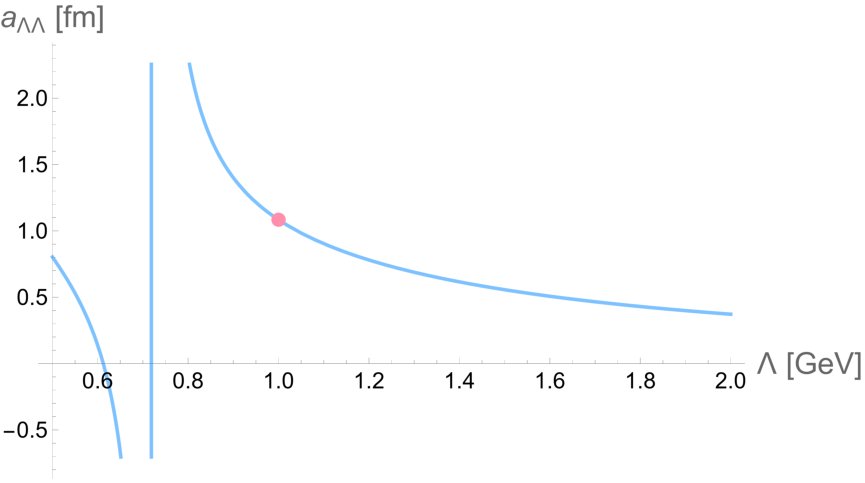
\includegraphics[width=\linewidth]{cutoff.pdf}
    \caption{Cutoff dependence of the $\Lambda\Lambda$ scattering length $a_{\Lambda\Lambda}$ in strategy~2 with $a_{NN}$ in $^3S_1$ as input. The dot marks the $a_{\Lambda\Lambda} = 1.1$~fm at cutoff $\Lambda = 1.0$~GeV. At $\Lambda = 0.72$~GeV, $a_{\Lambda\Lambda}$ reaches the unitarity limit.}
    \label{fig:cutoff}
    \end{center}
\end{figure}

Given the large scattering lengths, we now search for poles of the $T$-matrix on the complex energy plane across various Riemann sheets (RSs). For strategy~1 with $a_{NN}$ in $^3S_1$, the four channels are essentially decoupled (as seen from the values of $\tilde a$ and $\tilde b$), allowing separate single-channel analyses. The $\Sigma^*\Sigma^*$ channel exhibits a bound state, while the $\Lambda\Lambda$, $\Sigma\Sigma$, and $N\Xi$ channels each display a virtual state, as implied by the signs of the scattering lengths. Including coupled-channel effects produces negligible shifts of these poles. The results using $a_{NN}$ in $^1S_0$ are analogous. These pole positions are summarized in Table~\ref{tab:ES1}.

\begin{table}[tb]
\centering
\caption{Pole positions obtained using strategy~1 and single-channel analyses. The uncertainties include contributions from the $\Omega\Omega$ scattering length and from the cutoff dependence, estimated by scanning the cutoff $\Lambda$ from 2.0 to 0.5~GeV around the central value $\Lambda=1.0$~GeV. The subscript ``$\pm$'' denotes a pole on the first/second RS, corresponding to a bound/virtual state, respectively. }
\begin{tabular}{p{6em}cc}
\toprule
\multirow{2}{*}{} & \multicolumn{2}{c}{Strategy~1} \\
\cmidrule(lr){2-3}
& with $a_{NN}$ in $^3S_1$ & with $a_{NN}$ in $^1S_0$ \\
\midrule
$E_{\Lambda\Lambda}$ [GeV]
& $2.21\left(^{+0.01}_{-0.07}\right)_-$
& $2.21\left(^{+0.02}_{-0.08}\right)_-$ \\[5pt]
$E_{N\Xi}$ [GeV]
& $2.24\left(^{+0.02}_{-0.09}\right)_-$
& $2.23\left(^{+0.02}_{-0.10}\right)_-$ \\[5pt]
$E_{\Sigma\Sigma}$ [GeV]
& $2.38\left(^{+0.00}_{-0.02}\right)_-$
& $2.38\left(^{+0.01}_{-0.02}\right)_-$ \\[5pt]
$E_{\Sigma^*\Sigma^*}$ [GeV]
& $2.76\left(^{+0.00}_{-0.01}\right)_+$
& $2.77\left(^{+0.00}_{-0.02}\right)_+$ \\
\bottomrule
\end{tabular}
\label{tab:ES1}
\end{table}

For strategy~2 with $a_{NN}$ in $^3S_1$ as input, we find a total of thirty-two poles: two bound states and ten virtual states below the $\Lambda\Lambda$ threshold, along with ten complex-conjugate pairs of resonance poles between the $\Lambda\Lambda$ and $\Sigma^*\Sigma^*$ thresholds. Among these, two bound states and two resonance pairs are dominant, while the remaining twenty-six are shadow poles~\cite{Eden:1964zz}. The results using $a_{NN}$ in $^1S_0$ are analogous. We label the RSs as $(\pm,\pm,\pm,\pm)$, where the signs denote the imaginary parts of the channel momenta; bound states lie on the real axis of the physical sheet $(+,+,+,+)$. The dominant pole positions and their channel couplings are listed in Table~\ref{tab:ES2}.

\begin{table}[tb]
\centering
\caption{Four dominant poles and their coupling strengths to the scattering channels obtained using strategy~2. Here the RSs $(+,+,+,+)$, $(-,+,+,+)$, $(-,-,+,+)$, and $(-,-,-,+)$ are denoted as RS~I, II, III, and IV, respectively. Pole energies and coupling strengths are in units of GeV and GeV$^{-1/2}$, respectively. The uncertainties include contributions from the $\Omega\Omega$ scattering length and from the cutoff dependence, estimated by scanning the cutoff $\Lambda$ from 2.0 to 0.5~GeV around the central value $\Lambda=1.0$~GeV; the former is found to be numerically negligible compared to the latter. The cutoff dependence of the pole positions is also illustrated in Fig.~\ref{fig:trajectory}. Notably, the second pole in the RS~I moves to the RS~II as $\Lambda$ decreases; see its trajectory in Fig.~\ref{fig:trajectory}.}
\begin{tabular}{p{2em}cc}
\toprule
\multirow{2}{*}{} & \multicolumn{2}{c}{Strategy~2} \\
\cmidrule(lr){2-3}
&  with $a_{NN}$ in $^3S_1$ & with $a_{NN}$ in $^1S_0$ \\
\midrule
$E_{\rm I}^{(1)}$
& $2.13\left(^{+0.07}_{-0.11}\right)$
& $2.16\left(^{+0.06}_{-0.11}\right)$ \\[5pt]
$g_{\Lambda\Lambda}$
& $1.74\left(^{+0.06}_{-0.05}\right)$
& $1.71\left(^{+0.07}_{-0.19}\right)$ \\[5pt]
$g_{N\Xi}^{I=0}$
& $1.11\left(^{+0.16}_{-0.50}\right)$
& $1.03\left(^{+0.21}_{-0.63}\right)$ \\[5pt]
$g_{\Sigma\Sigma}^{I=0}$
& $1.91\left(^{+0.51}_{-0.88}\right)$
& $1.78\left(^{+0.58}_{-1.04}\right)$ \\[5pt]
$g_{\Sigma^*\Sigma^*}^{I=0}$
& $0.27\left(^{+0.07}_{-0.01}\right)$
& $0.28\left(^{+0.06}_{-0.04}\right)$ \\
\midrule
$E_{\rm I}^{(2)}$
& $2.22\left(^{+0.03-i0.003_{\rm II}}_{-0.09_{\rm I}}\right)$
& $2.23\left(^{+0.03-i0.003_{\rm II}}_{-0.09_{\rm I}}\right)$ \\[5pt]
$g_{\Lambda\Lambda}$
& $1.04\left(^{+2.84}_{-0.63}\right)$
& $0.78\left(^{+0.71}_{-0.67}\right)$ \\[5pt]
$g_{N\Xi}^{I=0}$
& $1.33\left(^{+8.27}_{-0.40}\right)$
& $1.20\left(^{+1.47}_{-0.97}\right)$ \\[5pt]
$g_{\Sigma\Sigma}^{I=0}$
& $0.80\left(^{+5.84}_{-0.18}\right)$
& $0.78\left(^{+1.15}_{-0.63}\right)$ \\[5pt]
$g_{\Sigma^*\Sigma^*}^{I=0}$
& $0.95\left(^{+3.00}_{-0.59}\right)$
& $0.76\left(^{+1.18}_{-0.64}\right)$ \\
\midrule
$E_{\rm III}$
& $2.47\left(^{+0.19}_{-0.08}\right)-i0.11\left(^{+0.28}_{-0.08}\right)$
& $2.46\left(^{+0.19}_{-0.07}\right)-i0.10\left(^{+0.27}_{-0.12}\right)$ \\[5pt]
$g_{\Lambda\Lambda}$
& $0.82\left(^{+0.01}_{-0.40}\right)$
& $0.82\left(^{+0.01}_{-0.38}\right)$ \\[5pt]
$g_{N\Xi}^{I=0}$
& $1.87\left(^{+1.15}_{-0.87}\right)$
& $1.81\left(^{+1.15}_{-0.96}\right)$ \\[5pt]
$g_{\Sigma\Sigma}^{I=0}$
& $2.30\left(^{+0.38}_{-0.51}\right)$
& $2.27\left(^{+0.38}_{-0.60}\right)$ \\[5pt]
$g_{\Sigma^*\Sigma^*}^{I=0}$
& $0.48\left(^{+1.19}_{-0.34}\right)$
& $0.45\left(^{+1.16}_{-0.34}\right)$ \\
\midrule
$E_{\rm IV}$
& $2.77\left(^{+0.12}_{-0.01}\right)-i0.07\left(^{+0.21}_{-0.05}\right)$
& $2.76\left(^{+0.11}_{-0.01}\right)-i0.06\left(^{+0.21}_{-0.05}\right)$ \\[5pt]
$g_{\Lambda\Lambda}$
& $0.95\left(^{+0.90}_{-0.53}\right)$
& $0.90\left(^{+0.93}_{-0.54}\right)$ \\[5pt]
$g_{N\Xi}^{I=0}$
& $0.64\left(^{+0.57}_{-0.35}\right)$
& $0.61\left(^{+0.59}_{-0.36}\right)$ \\[5pt]
$g_{\Sigma\Sigma}^{I=0}$
& $0.19\left(^{+0.18}_{-0.11}\right)$
& $0.18\left(^{+0.18}_{-0.11}\right)$ \\[5pt]
$g_{\Sigma^*\Sigma^*}^{I=0}$
& $1.96\left(^{+0.59}_{-0.45}\right)$
& $1.92\left(^{+0.63}_{-0.50}\right)$ \\
\bottomrule
\end{tabular}
\label{tab:ES2}
\end{table}

We now analyze the results in more detail, focusing exclusively on strategy~2 with $a_{NN}$ in the $^3S_1$ channel. A salient feature is the presence of strong coupled-channel effects. The $\Lambda\Lambda$ threshold lies at $2231.4$~MeV. The deeper bound state is located tens of MeV below it; within uncertainties, however, the binding energy may be as small as 10~MeV, compatible with the lower bound on the $H$ dibaryon mass reported in Ref.~\cite{Takahashi:2001nm}. This state couples strongly to the $\Lambda\Lambda$, $N\Xi$, and $\Sigma\Sigma$ channels (see the couplings in Table~\ref{tab:ES2}), indicating a pronounced multichannel character. The shallower bound state, which could become a resonance pole on the $(-,+,+,+)$ RS within uncertainties, lies closer to the $\Lambda\Lambda$ threshold and also near the $N\Xi$ threshold at around 2.26~GeV, coupling predominantly to the $N\Xi$ channel. Both poles can be regarded as members of the $S=-2$ $H$ dibaryon family. Notably, Ref.~\cite{Haidenbauer:2011ah} analyzed the $H$ dibaryon within chiral effective field theory and concluded that, if bound, it is more likely to be an $N\Xi$ bound state---a scenario also discussed in quark-model studies~\cite{Oka:1983ku, Nakamoto:1997gh}---with a binding energy of roughly 28~MeV relative to the $N\Xi$ threshold.

The resonance pole on RS $(-,-,+,+)$ couples most strongly to the $\Sigma\Sigma$ channel (see Table~\ref{tab:ES2}), with its imaginary part arising primarily from decays into the lower-lying channels. Notably, the real part of this pole lies above the $\Sigma\Sigma$ threshold. This can be understood as a consequence of the strong $N\Xi$-$\Sigma\Sigma$ coupling, which pushes this pole upward in energy while simultaneously driving the deeply bound state further down (for a general discussion, see Ref.~\cite{Zhang:2024qkg}). The resonance pole on RS $(-,-,-,+)$ can be interpreted as a $\Sigma^*\Sigma^*$ quasi-bound state, to which it couples predominantly. The $\Sigma^*\Sigma^*$ channel couples relatively weakly to the other three channels, as expected from the large mass gap between the spin-$3/2$ and spin-$1/2$ baryons, which leads to a partial decoupling.

Next, we examine the cutoff dependence of these four dominant poles by scanning $\Lambda$ from 2.0~GeV down to 0.5~GeV and tracing the pole trajectories on the RSs, as shown in Fig.~\ref{fig:trajectory}. For the two bound state poles on RS $(+,+,+,+)$, the binding becomes progressively shallower as the cutoff decreases. The shallower bound state reaches the $\Lambda\Lambda$ threshold at $\Lambda = 0.72$~GeV and, upon further reduction, moves onto RS $(-,+,+,+)$ as a virtual state. It then shifts along the negative real axis and eventually acquires an imaginary part, becoming a resonance---a clear indication that the attraction weakens with decreasing cutoff. For the two resonance poles on RS $(-,-,+,+)$ and $(-,-,-,+)$, their real parts decrease and both approach the real axis as the cutoff is lowered. This pattern can be understood as follows: decreasing the cutoff reduces the couplings between the lower and higher channel pairs, thereby weakening both the coupling-induced effective attraction in the $\Lambda\Lambda$ and $N\Xi$ channels and the coupling-induced effective repulsion in the $\Sigma\Sigma$ and $\Sigma^*\Sigma^*$ channels.

\begin{figure*}[tb]
    \centering
        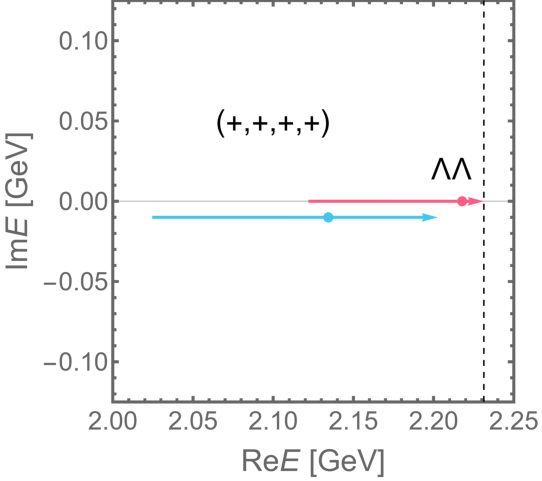
\includegraphics[height=4.cm]{I.pdf}\hfill
        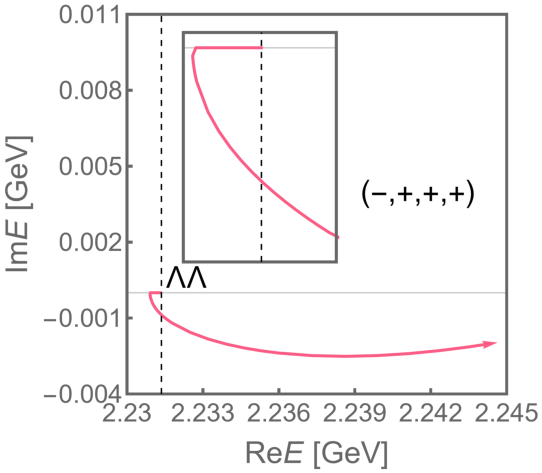
\includegraphics[height=4.cm]{II.pdf}\hfill
        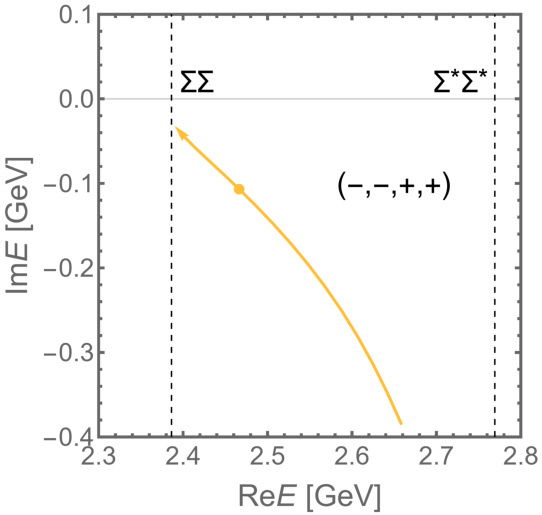
\includegraphics[height=4.cm]{III.pdf}\hfill
        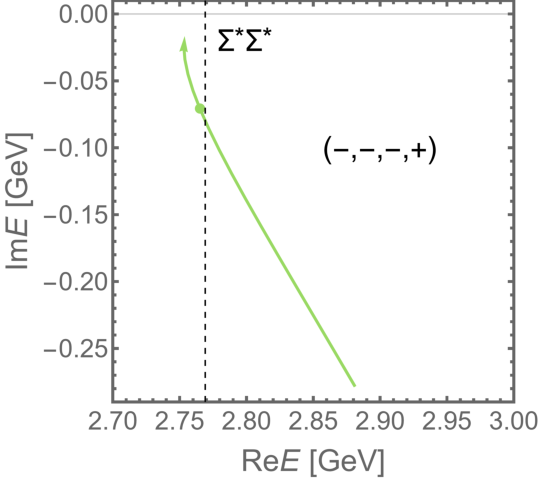
\includegraphics[height=4.cm]{IV.pdf}
    \caption{Trajectories of the four dominant poles in strategy~2 with $a_{NN}$ in $^3S_1$ as input, with arrows indicating decreasing the cutoff $\Lambda$ from 2.0~GeV to 0.5~GeV. Highlighted points mark the values at $\Lambda = 1.0$~GeV. On RS $(+,+,+,+)$, the deeper bound state is shifted slightly downward to avoid overlap with the shallower one. }
    \label{fig:trajectory}
\end{figure*}

Having clarified the analytic structure of the $T$-matrix, we now examine how these poles manifest in the $\Lambda\Lambda$ invariant mass spectrum. The invariant mass distribution for reactions induced via $i \to \Lambda\Lambda$ is proportional to
\begin{equation}
\Gamma_i=p_{\Lambda\Lambda}\left|T_{i\to\Lambda\Lambda}\right|^2,
\end{equation}
and the resulting lineshapes for the four channels are shown in Fig.~\ref{fig:ls}. A pronounced enhancement appears near the $\Lambda\Lambda$ threshold, arising from the lowest two poles. This feature is most prominent in the $\Lambda\Lambda \to \Lambda\Lambda$ channel, where the peak reaches its maximum around $2246$~MeV. In reactions with two $\Lambda$ hyperons in the final state, the $\Lambda\Lambda$ pair can proceed through all possible intermediate states before being observed, i.e., it can be produced via rescattering of other baryon pairs. In general, one expects that the $\Lambda\Lambda$ channel can be more easily produced than other $S=-2$ baryon pairs for several reasons: (1) the $\Lambda\Lambda$ threshold is the lowest; (2) forming an $N\Xi$ pair requires the two strange quarks to coalesce into a single $\Xi$, which demands a small relative momentum and is thus suppressed; (3) heavier hyperons decay into $\Lambda$. In such reactions, one expects to see a peak near the $\Lambda\Lambda$ threshold in the $\Lambda\Lambda$ invariant mass spectrum; as reported in the preliminary result of J-PARC E42 experiment~\cite{Ahn:2025exotic}.

Beyond the bound states, the two resonance poles also leave characteristic imprints on the invariant mass distributions. The lower-lying resonance couples most strongly to $\Sigma\Sigma$ and lies above the $\Sigma\Sigma$ threshold. Consequently, it produces a cusp at the $\Sigma\Sigma$ threshold in the other three lineshapes, manifesting either as a dip~\cite{Dong:2020hxe} or a peak. In the $\Sigma\Sigma\to\Lambda\Lambda$ transition, it generates an asymmetric enhancement that peaks below the $\Sigma\Sigma$ threshold and is strongly distorted and suppressed by the nearby threshold---a generic feature of resonances that are inaccessible on the physical RS in off-diagonal $T$-matrix elements~\cite{Zhang:2024qkg}. By contrast, the higher-lying resonance is unimpeded by the distant lower thresholds and thus appears as a clear peak in $\Gamma_{\Sigma^*\Sigma^*}$, while simultaneously inducing a pronounced dip in $\Gamma_{\Lambda\Lambda}$---a universality feature discussed in Ref.~\cite{Dong:2020hxe}.

\begin{figure}[tb]
    \begin{center}
    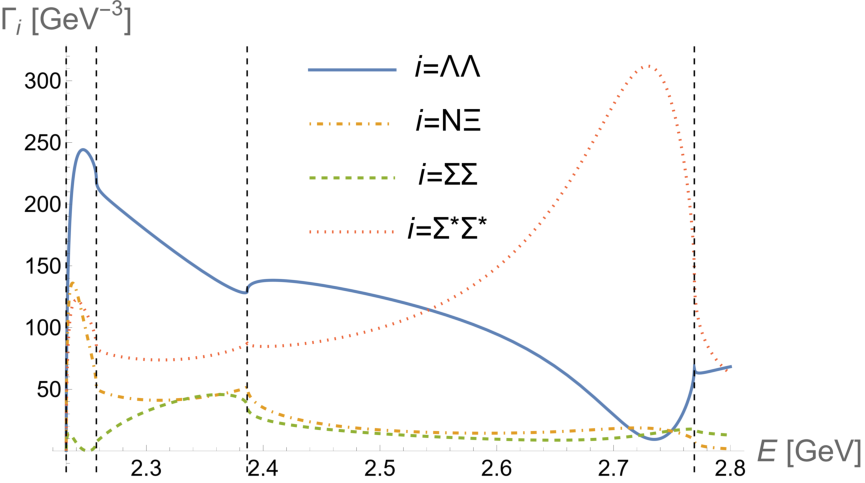
\includegraphics[width=\linewidth]{lineshape.pdf}
    \caption{Invariant mass distributions for the processes $\Lambda\Lambda$, $N\Xi$, $\Sigma\Sigma$, and $\Sigma^{*}\Sigma^{*}\to\Lambda\Lambda$ in strategy~2 with $a_{NN}$ in $^3S_1$, evaluated at cutoff $\Lambda = 1.0$~GeV. The vertical dashed lines indicate the four thresholds.}
    \label{fig:ls}
    \end{center}
\end{figure}

In conclusion, we have investigated the implications of SU(6) symmetry for $S$-wave baryon-baryon scattering in the $S=-2$ sector. Using an LO NREFT, the baryon-baryon interaction is constrained to two LECs, $\tilde{a}$ and $\tilde{b}$, enabling a predictive framework testable across multiple scattering channels. Focusing on the $J=0$, $Q=0$, $S=-2$ sector, which is of particular interest for the $H$ dibaryon, we find two bound states, consistent with the $H$ dibaryon manifesting as a multichannel state. There are also two higher poles located at about 2.47 and 2.77~GeV, respectively. In particular, the higher one should appear as a pronounced dip in the $\Lambda\Lambda$ invariant mass distribution of a reaction producing much more $\Lambda\Lambda$ than $\Sigma^*\Sigma^*$ pairs. These results offer new insights into exotic multibaryon dynamics and motivate further experimental searches for the $H$ dibaryon.

\begin{acknowledgements}
We thank Ulf-G. Mei{\ss}ner for a careful reading of the manuscript and helpful comments. This work is supported in part by the National Key R\&D Program of China under Grant No.~2023YFA1606703; by the National Natural Science Foundation of China under Grants No.~12125507, No.~12361141819, and No.~12447101; and by the Chinese Academy of Sciences under Grant No.~YSBR-101.
\end{acknowledgements}

\bibliography{refs}

\end{document}